\section{Implementarea modelului de recomandare}
\subsection{Inițializarea}
În implementarea prezentei aplicații este folosit framework-ul de construcție a sistemelor de recomandare $LightFM$ \hyperlink{lightfm}{[21]} peste s-a construit un wrapper. 
$LightFM$ conține o implemntare în Python a unor algoritmi de recomandare atât pentru feedback implicit cât și pentru feedback explicit. Metadatele filmelor și utilizatorilor pot fi încorporate intr-un algoritm tradițional de matrix factorization. Reprezentarea fiecărui film și utilizator este o sumă a reprezentărilor latente ale caracteristicilor, ceea ce îi permite să generalizeze recomandările și către filme sau utilizatori noi.   

În continuare este prezentată inițializarea modelului de recomandare și explicația parametrilor folosiți atât cei definiți ca fiind maleabili cât și ceilalți parametrii puși la dispoziție de framework dar asupra cărora nu s-a intervenit în prezenta implementare:
\begin{lstlisting}[language=Python, caption=Definirea modelului de recomandare]
from lightfm import LightFM

__all__ = ['KingRec']


class KingRec(object):
    def __init__(self, no_components=50, loss='warp', learning_rate=0.05, alpha=0.02, scale=0.07):
        self.no_components = no_components
        self.loss = loss
        self.learning_rate = learning_rate
        self.item_alpha = alpha
        self.user_alpha = alpha * scale
        
        self.model = LightFM(no_components=no_components, 
        					 learning_rate=learning_rate, loss=loss,
                             item_alpha=self.item_alpha, 
                             user_alpha=self.user_alpha, 
                             random_state=2019)                       
\end{lstlisting}

Parametrii maleabili:
\begin{itemize}
  \item \textbf{no\_components}: numărul de componente reprezintă dimensiunea encodării latente a caracteristicilor utilizatorilor și filmelor. Spre exemplu, numărul de caracteristici pe fiecare utilizator este de 1000 și avem 100 de utilizatori, ceea ce înseamnă o matrice de dimensiune $100 \times 1000$. Cu numărul de componente setat la 50, cum este prezentat în fragmentul de cod de mai sus, înseamnă ca numărul caracteristicilor pe fiecare utilizator va fi redus la 50 de unde rezultă noua matrice a encodărilor latente a caracteristicilor de dimensiune $100 \times 50$.
  \item \textbf{learning\_rate}: reprezintă rata de învățare de start pe care o folosește sistemul de recomandare. Această rată se poate schimba pe parcusul rulării ca urmare a faptului că s-a folosit algoritmul de optimizare Adagrad. Mai multe detalii despre acest algoritmi au fost prezentate în capitolul 2.2.3.
  \item \textbf{loss} funcția de eroare care poate fi una dintre următoarele funcții implementate: logistic, bpr, warp, warp-kos. Mai multe detalii despre funcțiile de eroare au fost prezentate în capitolul 2.1.3.
  \item \textbf{item\_alpha} penalizarea L2 norm a caracteristicilor articolelor. Este asignată direct din parametrul $alpha$.
  \item \textbf{user\_alpha} similar cu $item\_alpha$ și este rezultatul înmulțirii dintre parametrul $alpha$ și $scale$.
  \item \textbf{random\_state}: definește starea din care pleacă modelul de recomandare și este folosită de obicei pentru o reproducere mai ușoară a acelorași rezultate de la o rulare la alta.
\end{itemize}

Alți parametrii asupra carora nu s-a intervenit în prezenta implementare:
\begin{itemize}
	\item \textbf{k}: utilizat atunci când se folosește algoritmul k-OS și reprezintă al $k$-lea exemplu pozitiv ce va fi selectat din $n$ exemple pozitive pentru fiecare utilizator. Valoarea predefinită este setată la 5.
	\item \textbf{n}: utilizat atunci când se folosește algoritmul k-OS și reprezintă numărul maxim de exemple pozitive pentru fiecare actualizare. Valoarea predefinită este setată la 10.
	\item \textbf{learning\_schedule}: reprezintă algoritmul de optimizare și poate fi unul dintre adagrad sau adadelta. În experimentele realizate în această lucrare s-a folosit valoarea predefinită din model și anume adagrad.
	\item \textbf{max\_sampled}: reprezintă numărul maxim de exemple negative folosite în antrenarea cu WARP. Valoarea predefinită este setată la 10.
\end{itemize}

Odată definit modelul de recomandare putem crea o instanță a acestuia cu parametrii doriți dupa cum urmează:
\begin{lstlisting}[language=Python, caption=Instanțierea unui model]
from kingrec import KingRec

_, learning_rate, no_components, alpha, scaling = load_params(optimized_for='auc_clusters')

king_rec = KingRec(no_components=no_components, learning_rate=learning_rate, alpha=alpha, scale=scaling, loss='warp')
\end{lstlisting}
Această instanță va fi folosită în continuare în antrenarea și evaluarea modelului.
Funcția $load\_params$ încarcă parametrii optimi pentru pentru o anumită configurație. Mai multe detalii despre această optimizare a parametrilor este prezentată în capitolul 3.4.

\subsection{Antrenarea}
Cu o instanță a unui model creată putem antrena acel model pe un set de antrenare. Pentru a încărca un set de antrenare putem folosi funcția $init\_movielens$ care încarcă datasetul pus la dispoziție de grouplens \hyperlink{movielens}{[22]}. Mai multe detalii despre structura setului de date se pot găsi în capitolul 4.1.

\begin{lstlisting}[language=Python, caption=Funcția de inițializare a bazei de date]
def init_movielens(path, min_rating=0.0, k=3, item_features=None, cluster_n=18, model='vgg19')
\end{lstlisting}
unde:
\begin{itemize}
	\item \textbf{path}: este calea către folderul cu fișierele din setul de date;
	\item \textbf{min\_rating}: este ratingul minim pentru de la care vor fi construite interacțiunile dintre utilizatori și filme. Spre exemplu, dacă setăm un rating minim de $3.5$, mulțimea interacțiunilor pozitive va fi definită de acele interacțiuni pentru care utilizatorii au acordat cel puțin un rating de $3.5$, acestea fiind considerate interacțiuni pozitive. Restul interacțiunilor sunt considerate negative;
	\item \textbf{k}: este un parametru folosit doar pentru statisticii, în contextul de față prezintă câți utilizatori au minim $k$ interacțiuni în setul de date. Valoarea $k$ este folosită în metrica de evaluare $precizie@k$ după cum este prezentat în capitolul 3.1.1; 
	\item \textbf{item\_features}: poate lua una sau mai multe valori din mulțimea ${'genres', 'clusters'}$ și descrie tipurile de metadate ale filmelor care se doresc a fi prezente în setul de date. Desigur, acest parametru poate fi omis, astfel nefiind adăugate metadate suplimentare pe lângă interacțiunile dintre utilizatori și filme.
	\item \textbf{cluster\_n}: parametru folosit doar atunci când în $item\_features$ este prezentă valoarea $clusters$ și descrie în câte clustere trebuie să fie împărțite posterele filmelor. Clusterele sunt generate în prealabil și se găsesc în path-ul menționat;
	\item \textbf{model}: specifică modelul cu care au fost create posterele. Poate fi unul dintre următoarele: vgg19, inception\_v3, resnet50.
\end{itemize}
Funcția $init\_movielens$ returnează atât setul de date de antrenare cât și pe cel de testare. De asemenea, dacă este specificat prin parametrii returnează și metadatele filmelor.

Cu setul de date încarcat, putem face antrenarea cu funcția $fit$ sau $fit\_partial$. Diferența principală dintre cele două funcții este reprezentată de faptul că $fit\_partial$ reia antrenarea din starea curentă a modelului pe când $fit$ începe dintr-o stare nouă. 

\begin{lstlisting}[language=Python, caption=Antrenarea modelului]
model = king_rec.model
model.fit(interactions=train, item_features=item_features, epochs=epochs, verbose=True, num_threads=threads)
\end{lstlisting}
unde:
\begin{itemize}
	\item \textbf{interactions}: primește interacțiunile definite dintre utilizatori și filme;
	\item \textbf{item\_features}: reprezintă metadatele filmelor, dacă este cazul;
	\item \textbf{epochs}: reprezintă numărul de epoci pentru care vrem să facem antrenarea
	\item \textbf{verbose}: dacă este setat pe $True$ afișează progresul antrenării;
	\item \textbf{num\_threads}: numărul de threaduri pe care să fie executată antrenarea.
\end{itemize}

\subsection{Evaluarea}
Pe un model antrenat vom evalua două metrici pe setul de date de testare și anume \textit{acuratețea} și \textit{precizia@k}.
Prima dintre ele, \textit{acuratețea} este definită ca fiind probabilitatea ca un exemplu pozitiv ales în mod aleator să fie clasat mai sus în recomandări decât un exemplu negativ ales în mod aleator. Cea de-a doua, \textit{precizia@k} este definită de numărul de exemple pozitive aflate în primele $k$ recomandări.

Acuratețea poate fi calculată cu funcția $auc\_score$:
\begin{lstlisting}[language=Python, caption=Acuratețea unui model]
test_auc = auc_score(model, test_interactions, item_features=item_features, num_threads=threads).mean()
\end{lstlisting}
unde:
\begin{itemize}
	\item \textbf{model}: este modelul antrenat anterior;
	\item \textbf{test\_interactions}: reprezintă interacțiunile de test create cu funcția de inițializare a bazei de date;
	\item \textbf{item\_features}: reprezintă metadatele filmelor create cu funcția de intițializare a bazei de date;
	\item \textbf{num\_threads}: numărul de threaduri pe care se va executa evaluarea modelului.
\end{itemize}
Rezultatul produs este reprezentat de un scor de acuratețe pentru fiecare utilizator din setul de antrenare, iar rezultatul final al modelului este reprezentat de $mean$-ul tuturor rezultatelor de acuratețe per utilizator.

Precizia@k poate fi calculată cu funcția $precision\_at\_k$:

\begin{lstlisting}[language=Python, caption=Precizia@k a unui model]
test_precision = precision_at_k(model, test_interactions, item_features=item_features, k=k, num_threads=threads).mean()
\end{lstlisting}
unde:
\begin{itemize}
	\item \textbf{model, test\_interactions, item\_features și num\_threads}: descrise ca mai sus;
	\item \textbf{k}: numărul de recomandări peste care se calculează precizia pentru un utilizator.
\end{itemize}
Rezultatul produs este reprezentat de un scor de precizie@k pentru fiecare utilizator din setul de antrenare, iar rezultatul final al modelului este reprezentat de $mean$-ul tuturor rezultatelor de precizie per utilizator.

\section{Clusterizarea posterelor}
Procesul de clusterizare al posterelor presupune transformarea posterelor filmelor din imagini în clustere asociate fiecărui poster. Numărul total de clustere poate varia de la 2 până la 20 în cadrul acestei aplicații. De cele mai multe ori s-au folosit 18 clustere pentru a fi mapate 1 la 1 cu genurile filmelor.

Acest proces poate fi împărțit în două etape:
\begin{enumerate}
	\item Extragerea caracteristicilor din postere: în extragerea caracteristicilor din postere se folosesc mai multe rețele preantrenate printre care VGG16, VGG19, InceptionV3, ResNet50 sau NASNet. Mai multe detalii despre rețelele preantrenate pot fi găsite în capitolul 2.4. Folosim fiecare dintre rețelele menționate anterior până la stratul de clasificare, adică fără top-ul rețelelor, pentru a ne extrage doar caracteristicile din imagini. Imaginile în toate cele cinci rețele preantrenate întră cu dimensiunea fixă de $224 \times 224 \times 3$, inclusiv în rețeaua NASNet, chiar dacă aceasta poate accepta și dimensiuni mai mari. Fiecare film are câte un set de postere asociate, după cum este prezentat în capitolul 4.2. Din aceste seturi de postere alegem pentru fiecare film doar primul poster, poster pe care îl trecem prin fiecare dintre rețelele menționate mai sus. Odată trecut prin fiecare rețea, salvăm caracteristicile aferente fiecărei rețele într-un fișier specific. Aceste fișiere sunt formate din id-ul filmului și caracteristicile extrase de rețeaua specifică din primul poster al fimului.
Funcția care se ocupă de acest proces este $extract\_images\_features()$ din modulul $extract\_features.py$.
	\item Creeare clusterelor pe baza caracteristicilor posterelor: odată create fișierele cu caracteristici pentru fiecare rețea putem rula funcția $explore\_clusters()$ din modulul $create\_clusters.py$. În acest moment fiecare fișier de caracteristici va fi parcurs, iar pentru fiecare dintre aceste fișiere vom crea între 2 și 20 de clustere. La final, toate aceste clustere vor fi salvate într-un fișier asociat rețelei preantrenate. Spre exemplu, rulam funcția de creeare clustere pentru rețeaua preantrenată vgg19. Funcția va citi din fișierul asociate rețelei caracteristicile posterelor pentru fiecare film. Cu aceste caracteristici va genera $2, 4, 6, ..., 20$ de clustere. La final toate clusterele sunt salvate într-un fișier specific rețelei sub forma: id film, id poster, cluster 2 (unde va fi trecut în care cluster dintre cele două face parte posterul curent), cluster 4 (similar cu cluster 2), ..., cluster 20 (similar cu celelalte).
\end{enumerate}

\section{Construcția bazei de date}
Pentru construcția setului de date a fost folosită clasa \textit{Dataset} din framework-ul LightFM. Prima etapă în construirea bazei de date este citirea ratingurilor date de utilizatori filmelor. Odată citite ratingurile aplicăm filtrarea de minim rating, dacă este cazul. Ratingurile astfel rămase compun matricea de interacțiune. Se face un split de $80\%$ date de antrenare și $20\%$ date de testare pe aceste interacțiuni.

Pe parte de caracteristici, se folosesc prestabilit atât pentru utilizatori cât și pentru filme matrici de identitate. Spre exemplu, daca avem 500 de utilizatori și 1000 de filme vom avea matricea de caracteristici a utilizatorilor de dimensiune $500 \times 500$ având valoarea 1 pe diagonală, iar matricea de caracteristici a filmelor de dimensiune $1000 \times 1000$, având de asemenea valorea 1 pe diagonală.

În continuare, în funcție de parametrii setați în funcția \textit{init\_movielens} se încarcă și celelalte caracterstici specifice filmelor. Dacă avem setate genurile pentru a fi încărcate în matricea de caracteristici atunci pentru fiecare film vom citi din fișierul specific genurilor din setul de date genurile acestora. Un film poate avea unul sau mai multe genuri. Pentru a introduce aceste caracteristici în matricea de caracteristici vom aplica \textit{one hot encoding} ceea ce presupune că pentru o mulțime de genuri de dimensiune $n$ vom codifica mulțimea genurilor asociate unui film într-un vector de prezență de dimensiune $n$. Ceea ce înseamnă că dacă avem o mulțime de șapte genuri, fie ele genul 1, genul 2, ..., genul 7. Dacă un film are genul 3 și genul 7 atunci vectorul lui de caracteristici asociate genurilor va fi următorul $[0, 0, 1, 0, 0, 0, 1]$.

De asemenea funcția \textit{init\_movielens} poate inițializa și clusterele aferente fiecărui film. Procesul este similar cu cel definit mai sus pentru transferul genurilor filmelor în matricea de caracteristici.

Cu cele de mai sus definite propune un exemplu ce înglobează descrierea de mai sus:
Fie un set de date cu 500 de utilizatori și 1000 de filme. Numărul total de genuri este de 18. Numărul total de clustere este corelat cu numărul total de genuri, ceea ce înseamnă că vom avea un total de 18 clustere.
\begin{figure}[!h]
	\centering
	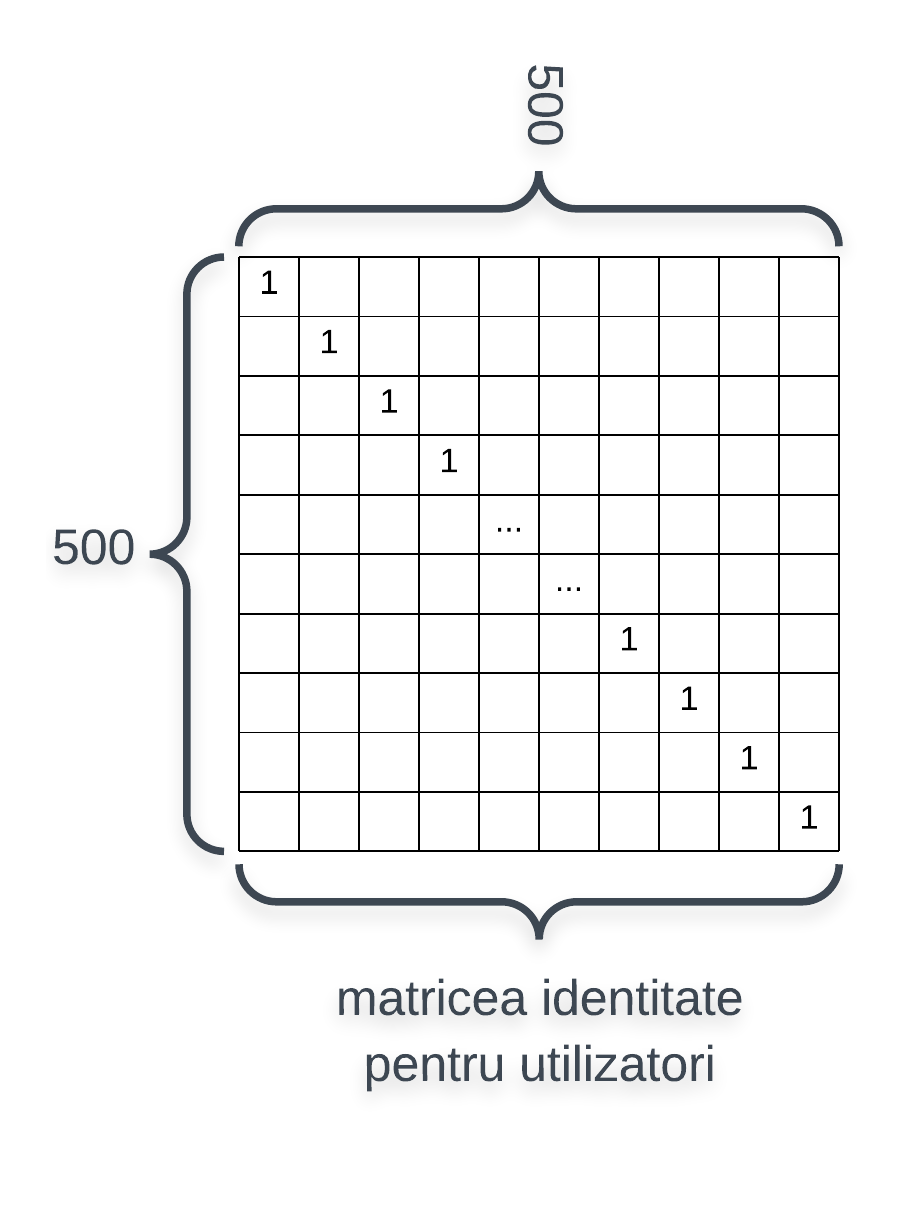
\includegraphics[max width=10cm,max height=10cm,keepaspectratio]{img_3_1}
	\caption[Structura setului de date pentru utilizatori]{Structura setului de date pentru utilizatori.}
\end{figure} 

\begin{figure}[!h]
	\centering
	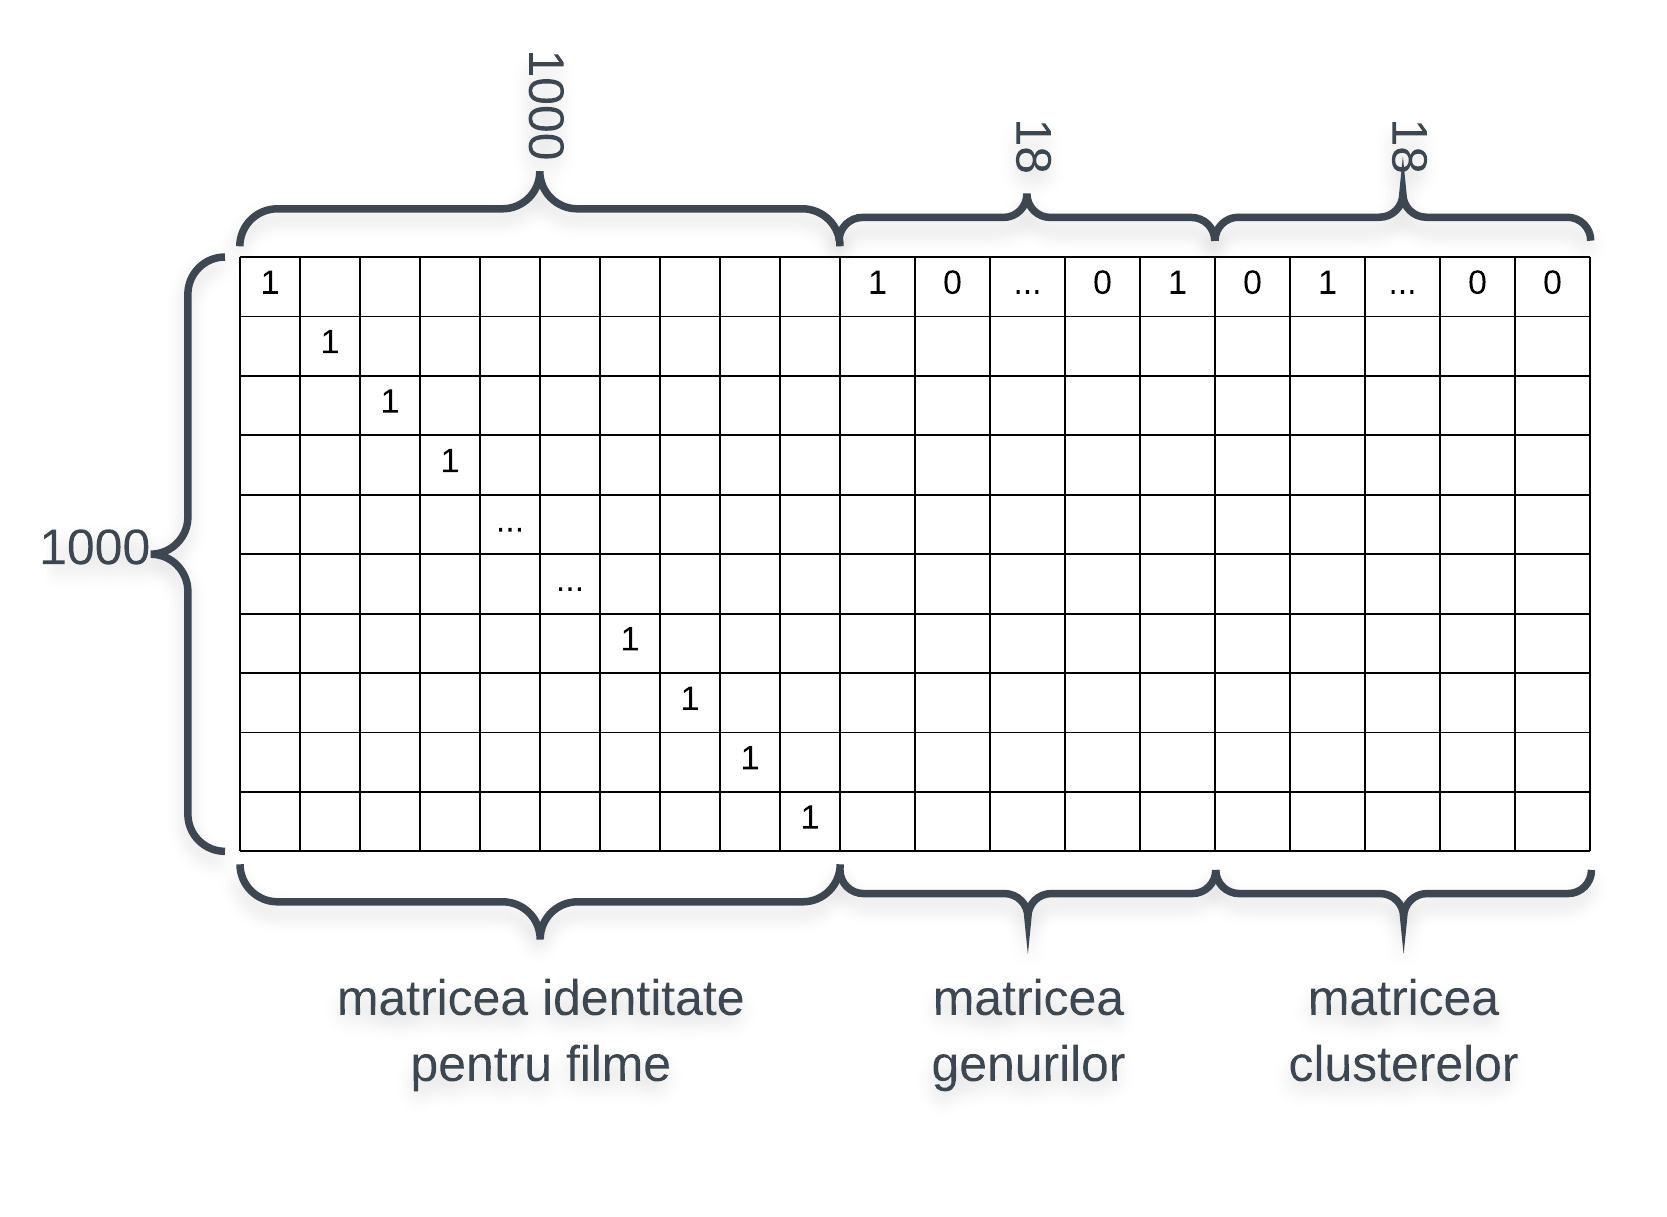
\includegraphics[max width=12cm,max height=12cm,keepaspectratio]{img_3_2}
	\caption[Structura setului de date pentru filme]{Structura setului de date pentru filme.}
\end{figure} 

\section{Optimizarea parametrilor modelului}
De multe ori în algoritmii de machine learning parametrii aleși precum rata de învățare sau numărul de epoci pot influența semnificativ rezultatul final. Astfel, pentru a reduce acest deficit există două variante: prima dintre ele presupune alegerea manuală a acestor parametrii prin diverse încercări; o a doua metodă presupune folosirea unor scripturi/librării specializate în minimizarea unor funcții definite fapt ce automatizează procesul de găsire a parametrilor optimi.

O astfel de librărie este folosită în prezenta lucrare de disertație și anume librăria skopt \hyperlink{skopt}{[22]}. Skopt este o librărie simplă și eficientă care minimizează funcții. Aceasta primește ca input o funcție de minimizat și un spațiu. Spațiul este definit ca fiind mulțimea parametrilor de optimizat și intervalele în care aceștia iau valori, spre exemplu:
\begin{lstlisting}[language=Python, caption=Spațiul parametrilor de optimizat]
space = [(1, 250),  # epochs
        (10 ** -4, 1.0, 'log-uniform'),  # learning_rate
        (20, 200),  # no_components
        (10 ** -6, 10 ** -1, 'log-uniform'),  # item_alpha
        (0.001, 1., 'log-uniform'),  # user_scaling
        (1, 5),  # k for k-OS training
        ] 
\end{lstlisting}

Un exemplu de funcție obiectiv de optimizare este următorea:
\begin{lstlisting}[language=Python, caption=Funcția obiectiv]
def objective(params):
    epochs, learning_rate, no_components, item_alpha, scale = params  # 'k_os'

    user_alpha = item_alpha * scale

    model = LightFM(loss=loss, random_state=2019, learning_rate=learning_rate,
                    no_components=no_components, user_alpha=user_alpha, item_alpha=item_alpha)
    model.fit(train, item_features=item_features, epochs=epochs, num_threads=threads, verbose=True)

    patks = function_to_optimize(model, test, item_features=item_features, num_threads=threads)
    mapatk = np.mean(patks)

    # Make negative because we want to minimize objective
    out = -mapatk

    # Handle some weird numerical shit going on
    if np.abs(out + 1) < 0.01 or out < -1.0:
        return 0.0
    else:
        return out
\end{lstlisting}
unde function\_to\_optimize poate fi una dintre funcțiile de precizie@k sau de acuratețe. De menționat că în cazul acestor două funcții o valoare mai bună înseamnă o valoare mai mare vom face outputul funcției obiectiv negativ astfel încât minimizând funcția obiectiv de fapt să aveam o valoare mai bună pentru funcția de precizie și acuratețe.

Scriptul a fost rulat pentru a optimiza parametrii modelului în următoarele situații:
\begin{enumerate}
	\item \textbf{fără metadate}
	\item \textbf{cu genuri}
	\item \textbf{cu clustere pe rețeaua vgg19, 18 clustere}
	\item \textbf{cu genuri și clustere pe rețeaua vgg19, 18 clustere}
	\item \textbf{cu clustere pe toate celelalte rețele preantrenate, 18 clustere}
	\item \textbf{cu genuri și clustere pe toate celelalte rețele preantrenate, 18 clustere}
\end{enumerate}
Rezultatele obținute se pot vedea în tabelele 3.1 și 3.2. Analizând cele două tabele putem trage următoarele concluzii, pe baza tabelului 3.1:
\begin{enumerate}
	\item funcția de eroare $warp$ obține cele mai bune rezultate atât pe precizie@k cât și pe acuratețe fie că alegem să folosim metadatele în orice combinație a lor, fie că alegem să nu le folosim, fapt pentru care în experimentele efectuate și relatate în tabelul 3.2 am ales să folosim doar această funcție de eroare;
	\item introducerea de metadate este clar o îmbunătățire față de varianta fără aceste metadate;
	\item există o corelație între genuri și clustere pe postere, rezultatele pe acuratețe și precizie fiind destul de apropiate;
	\item modelul de recomandare cu metadatele de clustere converge mai repede către un rezultat optim decât cu metadatele de genuri, atât pe precizie cât și pe acuratețe;
	\item folosite împreună, genurile și clusterele, se obține o îmbunătățire a sistemului de recomandare de aproximativ $1\%$ atât pe acuratețe cât și pe precizie față de modelul fără aceste metadate.
\end{enumerate}

Analizând tabelul 3.2 observăm următoarele:
\begin{enumerate}
	\item cea mai bună precizie și acuratețe pentru un model care folosește doar clustere a fost obținută cu clusterele create prin rețeaua resnet50;
	\item cea mai bună precizie atunci când se folosesc atât genurile cât și clusterele a fost obținută cu clusterele create prin rețeaua vgg19;
	\item cea mai bună acuratețe atunci când se folosesc atât genurile cât și clusterele a fost obținută cu clusterele create prin rețeaua inception\_v3.
\end{enumerate}

\begin{table}
\centering
\caption{Parametrii optimizați pentru modelul de recomandare pe tipuri de feature-uri}
\label{table:1}
\resizebox{\textwidth}{!}{\begin{tabular}{|c|c|c|c|c|c|c|c|c|c|} 
\hline
\multirow{2}{*}{\textbf{Features}} & \multirow{2}{*}{\textbf{Loss}} & \multirow{2}{*}{\textbf{Optimize}} & \multicolumn{6}{c|}{\textbf{Optimal params}}                                                                    & \multirow{2}{*}{\textbf{Results}}  \\ 
\cline{4-9}
                          &                       &                           & \textbf{epochs} & \textbf{learning rate}         & \textbf{no components} & \textbf{item alpha}             & \textbf{scaling}               & \textbf{k os} &                           \\ 
\hline
None                      & warp                  & precision\_at\_k          & 141    & 0.0430  & 21            & 0.0054    & 0.0147  &      & \textbf{0.0920}                    \\ 
\hline
None                      & warp                  & auc\_score                & 93     & 0.0131  & 169           & 2.6154143367150727e-06 & 0.0438   &      & \textbf{0.9309}                    \\ 
\hline
None                      & warp-kos~             & precision\_at\_k          & 131    & 0.0161  & 131           & 0.0148   & 0.0641     & 3    & 0.0915                    \\ 
\hline
None                      & warp-kos~             & auc\_score                & 136    & 0.0253  & 136           & 0.0253   & 0.0014 & 5    & 0.9123                    \\ 
\hline
None                      & bpr                   & precision\_at\_k          & 145    & 0.0118  & 145           & 0.0118   & 0.0087  &      & 0.0818                    \\ 
\hline
None                      & bpr                   & auc\_score                & 100    & 0.3833   & 22            & 0.3833    & 0.6705    &      & 0.8738                    \\ 
\hline
genres                    & warp                  & precision\_at\_k          & 136    & 0.0754     & 82            & 0.0070   & 0.0079   &      & \textbf{0.0990}                    \\ 
\hline
genres                    & warp                  & auc\_score                & 133    & 0.0262  & 193           & 0.0027  & 0.0732  &      & \textbf{0.9384}                    \\ 
\hline
genres                    & warp-kos              & precision\_at\_k          & 106    & 0.0458   & 200           & 0.0058   & 0.0973   & 5    & 0.0968                    \\ 
\hline
genres                    & warp-kos              & auc\_score                & 128    & 0.0313  & 103           & 5.6689548595143295e-06 & 0.2992    & 5    & 0.9184                    \\ 
\hline
genres                    & bpr                   & precision\_at\_k          & 4      & 0.3988    & 174           & 0.0002 & 0.9668    &      & 0.0793                    \\ 
\hline
genres                    & bpr                   & auc\_score                & 113    & 0.3787    & 20            & 1.412418076659026e-06  & 0.8846    &      & 0.8697                    \\ 
\hline
posters                  & warp                  & precision\_at\_k          & 63     & 0.0564   & 98            & 0.0031  & 0.0933    &      & \textbf{0.0938}                    \\ 
\hline
posters                  & warp                  & auc\_score                & 42     & 0.0570    & 68            & 0.0029  & 0.0256   &      & \textbf{0.9338}                    \\ 
\hline
posters                  & warp-kos              & precision\_at\_k          & 111    & 0.1214   & 30            & 0.0051   & 0.2238   & 3    & 0.0900                    \\ 
\hline
posters                  & warp-kos              & auc\_score                & 106    & 0.0206   & 153           & 0.0002  & 0.0172   & 5    & 0.9139                    \\ 
\hline
posters                  & bpr                   & precision\_at\_k          & 112    & 0.0278   & 53            & 0.0430   & 0.0450  &      & 0.0794                    \\ 
\hline
posters                  & bpr                   & auc\_score                & 76     & 0.3969   & 20            & 3.559358324483847e-05  & 0.7491     &      & 0.8656                    \\ 
\hline
genres, posters          & warp                  & precision\_at\_k          & 96     & 0.1703    & 22            & 0.0042   & 0.0413  &      & \textbf{0.0980}                    \\ 
\hline
genres, posters          & warp                  & auc\_score                & 120    & 0.0277  & 189           & 0.0011  & 0.4922    &      & \textbf{0.9406}                    \\ 
\hline
genres, posters          & warp-kos              & precision\_at\_k          & 83     & 0.0748   & 190           & 0.0079   & 0.0124  & 5    & 0.0916                    \\ 
\hline
genres, posters          & warp-kos              & auc\_score                & 149    & 0.0374    & 98            & 6.392983080540728e-05  & 0.6204    & 5    & 0.9205                    \\ 
\hline
genres, posters          & bpr                   & precision\_at\_k          & 19     & 0.0012 & 140           & 9.939007330655304e-05  & 0.0011 &      & 0.0597                    \\ 
\hline
genres, posters          & bpr                   & auc\_score                & 98     & 0.3429    & 21            & 8.687526249607698e-06  & 0.7296    &      & 0.8681                    \\
\hline
\end{tabular}}
\end{table}

\begin{table}
\centering
\caption{Parametrii optimizați pentru modelul de recomandare pe tipuri de feature-uri și modele de rețele preantrenate}
\label{table:2}
\resizebox{\textwidth}{!}{\begin{tabular}{|c|c|c|c|c|c|c|c|c|c|} 
\hline
\multirow{2}{*}{\textbf{Features} } & \multirow{2}{*}{\textbf{Loss }} & \multirow{2}{*}{\textbf{Optimize} } & \multicolumn{5}{c|}{\textbf{Optimal params}}                                                                      & \multirow{2}{*}{\textbf{Model} } & \multirow{2}{*}{\textbf{Results }}  \\ 
\cline{4-8}
                                    &                                 &                                     & \textbf{epochs} & \textbf{learning rate} & \textbf{no components} & \textbf{item alpha}   & \textbf{scaling}      &                                  &                                     \\ 
\hline
posters                            & warp                            & precision\_at\_k                    & 232             & 0.0717    & 42                     & 0.0065  & 0.0161  & vgg19                            & 0.0935                              \\ 
\hline
posters                            & warp                            & auc\_score                          & 89              & 0.0188   & 139                    & 0.0008 & 0.2864    & vgg19                            & 0.9325                              \\ 
\hline
genres, posters                    & warp                            & precision\_at\_k                    & 218             & 0.1247    & 73                     & 0.0054  & 0.0463   & vgg19                            & \textbf{0.0995}                              \\ 
\hline
genres, posters                    & warp                            & auc\_score                          & 236             & 0.0318   & 139                    & 0.0010 & 0.8362    & vgg19                            & 0.9413                              \\ 
\hline
posters                            & warp                            & precision\_at\_k                    & 119             & 0.0085    & 192                    & 7.276515301192984e-05 & 0.0270  & inception\_v3                    & 0.0836                              \\ 
\hline
posters                            & warp                            & auc\_score                          & 232             & 0.0298    & 84                     & 0.0042  & 0.0405  & inception\_v3                    & 0.9327                              \\ 
\hline
genres, posters                    & warp                            & precision\_at\_k                    & 245             & 0.0289   & 43                     & 0.0006 & 0.3657   & inception\_v3                    & 0.0905                              \\ 
\hline
genres, posters                    & warp                            & auc\_score                          & 250             & 0.0194   & 136                    & 0.0008 & 0.4767    & inception\_v3                    & \textbf{0.9425}                              \\ 
\hline
posters                            & warp                            & precision\_at\_k                    & 88              & 0.0749    & 21                     & 0.0046  & 0.0281  & resnet50                         & \textbf{0.0953}                              \\ 
\hline
posters                            & warp                            & auc\_score                          & 198             & 0.0167   & 169                    & 0.0012 & 0.6692    & resnet50                         & \textbf{0.9342}                              \\ 
\hline
genres, posters                    & warp                            & precision\_at\_k                    & 224             & 0.0421    & 186                    & 0.0086  & 0.0024 & resnet50                         & 0.0970                              \\ 
\hline
genres, posters                    & warp                            & auc\_score                          & 211             & 0.0976    & 48                     & 0.0034  & 0.1123   & resnet50                         & 0.9397                              \\
\hline
\end{tabular}}
\end{table}

În capitolul următor sunt utilizați acești parametrii optimi găsiți pentru a studia evoluția performanței modelului în timp, studiu ce ne va permite să tragem concluziile finale.